\subsection{Rapid Test Demand}
\label{subsec:rapid_test_demand}

In our model, there are five reasons why rapid tests are done:\comment[id=J]{ Add a
    section on how we calibrate rapid test demand; Mainly describe the datapoints we have
    and say that we usually interpolate linearly in between data points. (Only exception
    to that is private rapid test demand, which we fit to data)
}

\begin{enumerate}
    \item someone plans to have work contacts
    \item someone is an employee of an educational facility or a school pupil
    \item a household member has tested positive or developed symptoms
    \item someone has developed symptoms but has not received a PCR test
    \item someone plans to participate in a weekly non-work meeting
\end{enumerate}

%%% \subsubsection{work rapid tests}

For work contacts, we know from the COSMO study (\cite{Betsch2021}, 20th/21st of April)
that 60\% of workers who receive a test offer by their employer regularly use it. We
assume this share to be time constant.

In addition, there are some surveys that allow us to trace the expansion of employers who
offer tests to their employees. Mid march, 20\% of employers offered tests to their
employees \citep{DIHK2021}. In the second half of March, 23\% of employees reported being
offered weekly rapid tests by their employer \citep{Ahlers2021}. This share increased to
61\% until the first days of April \citep{BMWI2021, IZA2021}.

Until mid April 72\% of workers were expected to receive a weekly test offer
\citep{BMWI2021, IZA2021}. However, according to surveys conducted in mid April
\citep{Betsch2021}, less than two thirds of individuals with work contacts receive a test
offer. Starting on April 19th employers were required by law to provide two weekly tests
to their employees \citep{Bundesanzeiger2021}. We assume that compliance is incomplete
and only 80\% of employers actually offer tests. We interpolate between these points
linearly, arriving at the blue line in Figure~\ref{fig:rapid_test_demand}.

%%\subsubsection{educ rapid tests}

We assume that employees in educational facilities start getting tested in 2021 and that
by March 1st 30\% of them are tested weekly. The share increases to 90\% for the week
before Easter. At that time both Bavaria \citep{STMGP2021} and Baden-Württemberg
\citep{MinisteriumKultus2021} were offering tests to teachers and North-Rhine Westphalia
\citep{SchulministeriumNRW2021} and Lower Saxony \citep{NSMK2021} were already testing
students and tests for students and teachers were already mandatory in Saxony
\citep{SMK2021}. After Easter we assume that 95\% of teachers get tested twice per week.

Tests for students started later \citep{MinisteriumKultus2021, SchulministeriumNRW2021}
so we assume that they only start in February and only 10\% of students get tested by
March 1st. Relying on the same sources as above we approximate that by the week before
Easter this share had increased to 40\% \citep{SchulministeriumNRW2021}.

After Easter the share of students receiving twice weekly tests is set to 75\%. This is
based on tests becoming mandatory in Bavaria \citep{BayerischeStaatskanzlei2021} and
North Rhine-Westphalia \citep{SchulministeriumNRW2021b} after their Easter breaks and on
the 19th in Baden-Württemberg \citep{KMBaWue2021}. Again, we interpolate linearly between
these points and arrive at the purple line for teachers and the red line for school
students in Figure~\ref{fig:rapid_test_demand}.

%%\subsubsection{private rapid tests}

To limit our degrees of freedom, we only have one parameter that governs how many
individuals do a rapid test because of any of the private demand reasons (own symptoms
but no PCR test, planned weekly leisure meeting or a symptomatic or positively tested
household member).

We assume that there is no private rapid test demand until March when both the citizens'
tests and rapid tests for lay people started to become available
\citep{Bundesanzeiger2021a, Bundesregierung2021} and other access to rapid tests was very
limited.

According to the COSMO study \citep{Betsch2021a} 63\% would have been willing to take a
test in the round of 23rd of February 2021 when an acquaintance would have tested
positive. Since this is only asking for willingness not actual behavior, we take this as
the upper bound of private rapid test demand which we estimate in our model to be reached
in the beginning of May. To cover that many people are likely to have sought and done
their first rapid test before the Easter holidays we add another point that we estimate
for the rapid test demand around Easter. Similarly, we estimate one point in mid March
when tests started to become available in grocery stores and pharmacies which we estimate
in our model. The resulting share of private rapid test demand is shown as the green line
in Figure~\ref{fig:rapid_test_demand}.


\begin{figure}
    \centering
    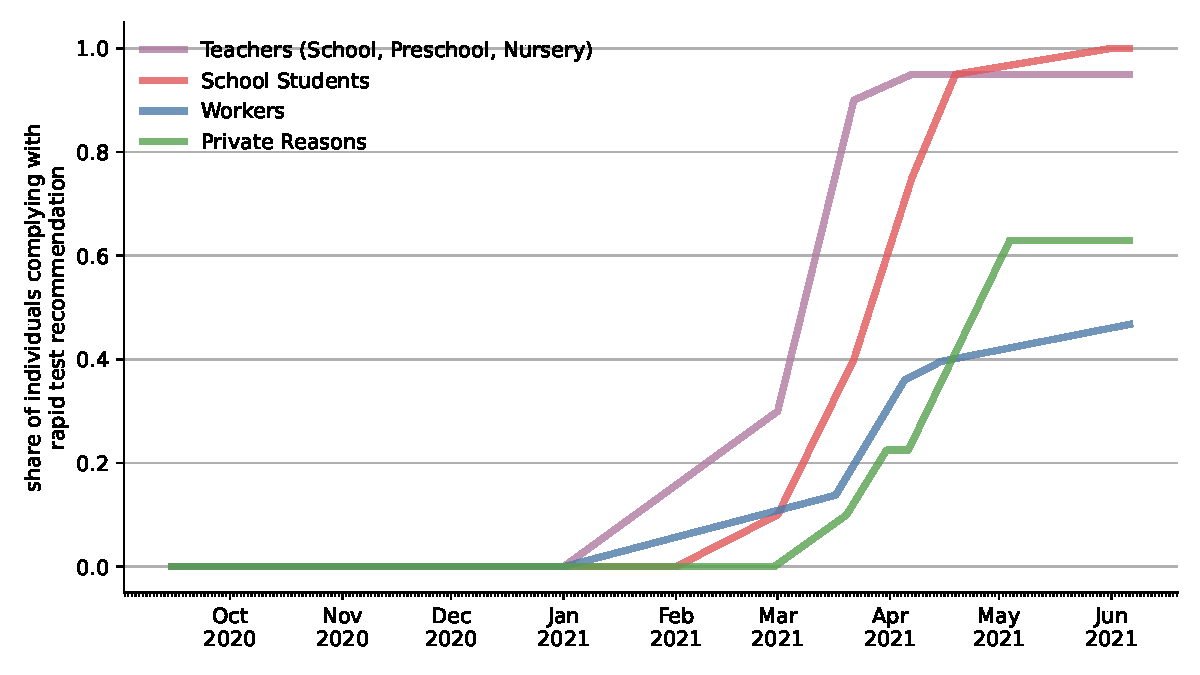
\includegraphics[width=0.5\textwidth]{figures/results/figures/data/testing/rapid_test_demand/baseline_shares}
    \caption{Share of Individuals Doing a Rapid Test.}
    \floatfoot{\noindent \textit{Note:} Rapid test demand can be triggered by individuals
    planning to have education contacts, work contacts, developing symptoms without
    access to a PCR test, having a household member with a positive test or symptoms. In
    each case whether a rapid test is done depends on how long it has been since the
    individual's last rapid test and her individual compliance parameter. As an example,
    take a worker in May. In that time workers are encouraged to test themselves twice
    weekly but there is no general requirement to test themselves. If the worker has not
    done a test within the last four days in our model she will demand a test if her
    (time-constant) compliance parameter belongs to the upper 60\% in the population.}
    \label{fig:rapid_test_demand}
\end{figure}

\FloatBarrier